\scanpage{73}
\mspage{32}
14. \uline{Description heuristique des} $\Sigma_i,\Sigma_{ij}$.
(Peut se préciser considérablement \unsure{ds|dans} un contexte de topologie modérée).
Pour construire $\Sigma_i$, on prend un voisinage tubulaire
\inserted{``standart'' $T_{<i}$} \deleted{\unsure{fermé}} de
$\unsure{\dot X_i|\dot\Sigma_i}=\displaystyle\bigcup_{k<i}X_k$, et on prend
\[
(42)\qquad\Sigma_i=X_i\setminus X_i\cap\mathring T_{<i}.
\]
\[
\mathring T_{<i}\overset{\mathrm{déf}}{=}T_{<i}\setminus\dot T_{<i}.
\]
\margin{\uline{NB} On peut prendre $T_{<i}=\bigcup_{k<i}T_k$,
où $T_k$ est un vois. tub. standart des $X_k$}
(\uline{NB} Il aurait suffit ici de prendre le voisinage tubulaire
standart dans $X_i$ lui $\unsure{\overline{\mathrm m}}$, et de prendre donc
$\Sigma_i=X_i\setminus\mathring T_{<i}$)

Pour construire $\Sigma_{ij}$, on prend un voisinage tubulaire
$T'_{ij}$ de $\Sigma_i$ dans
$X_j\setminus X_j\cap\unsure{\mathring T_{<i}|\mathring T_{<i0}}=X'_i$
(NB cette fois-ci il faut \deleted{prendre} d'abord prendre
$T_{<i}$ vois. tub. standart \uline{ds} $X$, ou sinon, ds $X_j$).
On prend $T'_{ij}$ ``suffisamment petit'' p.r. au choix de $T_{<i}$.
Puis on prend $\dot T'_{ij}$\deleted{\unsure{s}}, et dans $\dot T'_{ij}$
la trace de $\displaystyle\bigcup_{\unsure{i<k<j|i\leq k<j}}\unsure{X_{jk}|X_k}$
(\unsure{donc c'est} vide si $j$ est un successeur de $i$), soit $S\dot T'_{ij}$
(``partie singulière'' de $T'_{ij}$.

\figure{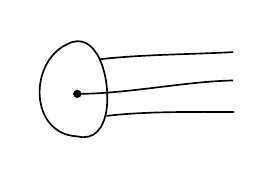
\begin{tikzpicture}[x=1cm,y=1cm,line width=.6pt]
\draw (0.05,-.58) .. controls (-.56,-.55) and (-.57,.36) .. (-.08,.59)
.. controls (.29,.79) and (.48,.18) .. (.42,-.25)
.. controls (.38,-.49) and (.26,-.63) .. (.05,-.58);
\draw (.34,.40) .. controls (.87,.46) and (1.45,.46) .. (2.03,.49);
\draw (.06,-.04) .. controls (.68,-.04) and (1.44,.12) .. (2.03,.13);
\draw (.42,-.32) .. controls (.92,-.26) and (1.55,-.27) .. (2.04,-.27);
\fill (.05,-.04) circle (1.5pt);
\end{tikzpicture}}

On prend alors un voisinage tubulaire standart
\inserted{$T(S\dot T'_{ij})$} de $S\dot T'_{ij}$ dans $\dot T'_{ij}$,
qu'on peut supposer induit par la réunion \inserted{$\bigcup T_k$}
des voisinages tubulaires standart des $X_k$ ($i<k<j$)
dans $\unsure{X---X_j}$
(pris ``assez petits'' p.r. aux choix déjà faits de $T_{<i}$
et \inserted{de} $T'_{ij}$).
On \deleted{\unsure{prendra}}\inserted{aura} alors
\[
(43)\qquad\Sigma_{ij}=\dot T'_{ij}\setminus\mathring T(S\dot T'_{ij})
\]
\mspage{72}
